\documentclass[a4paper,12pt]{book}
\usepackage[utf8]{inputenc}
\usepackage{graphicx}
\usepackage[square,numbers]{natbib}
\usepackage{float}
\usepackage{enumitem}
\usepackage{amsmath}
\usepackage{amssymb}
\usepackage{hyperref}
\usepackage{booktabs}
\usepackage{setspace}
\usepackage{geometry}
\usepackage[italian]{babel}
\usepackage{tikz}
\usepackage{pdfpages}
\usetikzlibrary{arrows}
\usetikzlibrary{backgrounds}
\bibliographystyle{unsrtnat}
\usepackage{booktabs}
\usepackage[normalem]{ulem}
\usepackage{listings}
\usepackage{fancybox}
\usepackage{xcolor}
\usepackage{inconsolata}

\definecolor{dkgreen}{rgb}{0,.6,0}
\definecolor{dkblue}{rgb}{0,0,.6}
\definecolor{dkyellow}{cmyk}{0,0,.8,.3}
\definecolor{dkblue}{rgb}{0, 0, 254}

\lstset{
	language        = php,
	frame			= single,
	captionpos		= b,
	basicstyle      = \small\ttfamily,
	keywordstyle    = \color{dkblue},
	stringstyle     = \color{red},
	identifierstyle = \color{black},
	commentstyle    = \color{gray},
	emph            =[1]{php},
	emphstyle       =[1]\color{black},
	emph            =[2]{public,if,and,null,or,else,foreach,return,as},
	emphstyle       =[2]\color{violet},
	emph			=[3]{show, up, store, index},
	emphstyle       =[3]\color{orange},
	emph			=[4]{Route,middleware,get,post,Blueprint,Schema,create,function, Note,Location,File, Video,find,sqrt,Response,pow,forget,Storage, disk, put, Request},
	emphstyle       =[4]\color{cyan},	
}


\begin{document}
	
	\includepdf{/Users/Ribbo/Desktop/Laurea/Tesi/frontespizioTesi.pdf}
	
	\tableofcontents
	
	\frontmatter
	
	\mainmatter
	
	\chapter*{Introduzione}



In un mondo sempre più urbanizzato e in cui la popolazione invecchia sempre di più, le città sono un punto di incontro per la società contemporanea. Per questo motivo è sorta la necessità di iniziare a pensare a quali requisiti debba avere una città del futuro. Per venire incontro a questo fenomeno si è introdotto il concetto di \textit{\textbf{walkability}}. Generalmente, il termine walkability indica il livello di sicurezza e comfort per i pedoni in una certa area urbana. Concretamente, una città ha un buon livello di walkability se le strade e i marciapiedi presenti sono in buono stato, se è presente una segnaletica stradale chiara e se sono presenti negozi per ogni tipo di necessità ad una distanza facilmente percorribile a piedi.

Il progetto Urban Story Sharing nasce da un'idea del Dipartimento di Informatica, Sistemistica e Comunicazione dell'Università degli studi di Milano-Bicocca, che ha come obiettivo quello di migliorare la walkability delle aree urbane, attraverso un'applicazione mobile che permette ai cittadini di raccogliere dati relativi ai centri urbani da loro frequentati, descrivendo storie attraverso note, immagini, audio e video. Le annotazioni geolocalizzate verranno salvate su un repostory centralizzato così da poter essere condivise fra utenti. Questo progetto si focalizza, invece, sulla realizzazione di un web service per la raccolta e la distribuzione delle storie urbane, supporterà quindi due delle operazioni \textbf{CRUD} base, quali GET e POST. 
La realizzazione del sistema è stata suddivisa in due parti, lo sviluppo del \textit{\textbf{front-end}} e lo sviluppo del \textit{\textbf{back-end}}.
In questo lavoro di stage si illustrerà la parte di sviluppo del \textit{\textbf{back-end}}.
Con il termine back-end, ci si riferisce ad applicativi software con i quali gli utenti interagiscono indirettamente, solitamente attraverso l'utilizzo di applicazioni front-end.

Nei prossimi capitoli verrà presentato il progetto in ogni sua parte, dalla fase di progettazione a quella di implementazione.  In particolare, nel capitolo 1 si analizzeranno le tecnologie utilizzate per la realizzazione del servizio web. Nel capitolo 2 verrà illustrata la fase di progettazione. Nel capitolo 3 verranno esposte le scelte implementative del progetto. Infine, nel capitolo 4 saranno presentate le conclusioni e gli sviluppi futuri.


	\chapter{Tecnologie utilizzate}

Questo capitolo si concentrerà solo sulle funzionalità offerte dal framework utilizzate durante la realizzazione dei servizi web per la raccoltà dei dati.

\section{Laravel}
Laravel è un framework per lo sviluppo di applicazioni web che cerca di facilitare il processo di sviluppo, semplificando le attività ripetitive utilizzate nella maggior parte delle applicazioni Web di oggi.
Dal momento che riesce a fare tutti i compiti essenziali che vanno dalla gestione del web e gestione del database alla generazione di codice HTML, Laravel è chiamato \textbf{full stack framework}. Questo ambiente di sviluppo web integrato è pensato per offrire un miglioramento nel flusso di lavoro dello sviluppatore.

A differenza di altri ambienti di sviluppo, Laravel necessita solo di qualche modifica al codice di configurazione PHP ed è pronto per l'uso. Inoltre, l'utilizzo di pochi file di configurazione consente alle applicazioni web Laravel di avere un struttura del codice simile che le rende molto caratteristiche e facilmente identificabili. D'altro canto questo potrebbe essere visto come un vincolo su come lo sviluppatore intende organizzare la propria appliczione. Tuttavia, questi vincoli rendono molto più facile e veloce la creazione di applicazioni Web. Inoltre offre una macchina virtuale, \textbf{Laravel Homestead}, Vagrant pre-confezionata che fornisce un ambiente di sviluppo senza che sia necessario installare PHP, un server Web e qualsiasi altro software server sul computer locale. Le virtual machine di Vagrant sono completamente usa e getta quindi se qualcosa va storto, la si puo distruggere e ricreare in pochi minuti.

In questo progetto le funzionalità utilizzate di Laravel sono l'Eloquent ORM, i model, le route, i controller e i database.

\subsection{ORM: Object-Relational Mapping}
L'ORM è una tecnica di programmazione che aiuta a convertire i dati tra sistemi incompatibili.
A questo scopo, Laravel, fornisce \textbf{Eloquent ORM} che consente di lavorare con gli oggetti e le tabelle del database utilizzando una sintassi semplice ed intuitiva. Ogni tabella del database ha un \textbf{modello} corrispondente utilizzato per l'interazione con quella tabella. 

\subsection{Model}
Un Model è lo strumento con cui lo sviluppatore può manipolare i dati. Può essere considerato uno strato collocato tra i dati e l'applicazione.

\subsection{Route}
Le route permettono di definire gli instradamenti delle richieste HTTP. La loro funzione base è quella di definire come va gestita una certa richiesta HTTP. Avendo utilizzato in questo progetto delle classi Controller, le route si limiteranno a instradare le varie richieste verso l'opportuno controller.

\subsection{Controller}
Come anticipato nella sezione 1.1, Laravel semplifica molte operazioni. I controller fanno parte di queste semplificazioni permettendo di raggruppare ed organizzare tutta la logica di gestione delle richieste HTTP. I controller possono raggruppare la logica di gestione delle richieste correlate in una singola classe.

\subsection{Database}
L'interazione con i database offerta dal framework può essere strutturata in 3 parti:
\begin{itemize}
	\item \textbf{Eloquent ORM}
	
	L'ORM Eloquent fornito con Laravel include una semplice implementazione PHP ActiveRecord che consente allo sviluppatore di eseguire query di database con una sintassi PHP invece di scrivere codice SQL, i metodi vengono semplicemente concatenati. Ogni tabella nel database possiede un Modello corrispondente attraverso il quale lo sviluppatore interagisce con detta tabella.
	
	\item \textbf{Schema builder}
	
	La classe Laravel Schema fornisce un database in grado di funzionare con una moltitudine di DBMS per gestire tutto il lavoro relativo al database come la creazione o l'eliminazione di tabelle o l'aggiunta di campi a una tabella esistente. Funziona con una moltitudine di sistemi di database supportati da Laravel e MySQL.
	
	\item \textbf{Migrations}
	
	Le migrazioni possono essere considerate come un controllo di versione per il nostro database, infatti, consentono di modificare lo schema del database, descrivere e registrare tutte quelle modifiche specifiche in un file di migrazione. Ogni migrazione viene solitamente associata a un generatore di schemi per gestire il tutto senza sforzo. Una migrazione può anche essere ripristinata o riportata ad una versione precedente.
	
	\item \textbf{Seeders}
	
	La classe Seeder consente di inserire i dati nelle nostre tabelle. Questa funzione è molto utile poiché lo sviluppatore può inserire dati fittizzi nelle tabelle del database ogni volta che desidera testare l'applicazione web.
	
\end{itemize}

\section{Composer}

Un'altra caratteristica che distingue Laravel dagli altri framework è che è un framework Composer ready. In effetti, Laravel è esso stesso una miscela di diversi componenti Composer, ciò aggiunge un'interoperabilità al framework.
Composer è uno strumento di gestione delle dipendenze per PHP. Essenzialmente, il ruolo principale di Composer nel framework di Laravel è quello di gestire la dipendenza delle dipendenze del nostro progetto. Ad esempio, se una delle librerie che stiamo utilizzando nel nostro progetto dipende da altre tre librerie che devono essere aggiornate, non è necessario trovare e aggiornare manualmente alcun file. È possibile aggiornare tutte e quattro le librerie tramite un singolo comando.
Un altro vantaggio nell'utilizzo di Composer è che genera e gestisce un file di caricamento automatico, \textbf{autoload}, nella radice della directory \textbf{vendor/}, che conterrà tutte le dipendenze del progetto. In tal modo, dal lato dello sviluppatore non è necessario ricordare tutti i percorsi delle dipendenze e includere ciascuno di essi in ogni file del progetto, deve solo includere il file \textbf{autoload} fornito da Composer. 

\pagebreak
\section{Artisan}
Uno sviluppatore dovrebbe solitamente interagire con il framework di Laravel usando un'utilità a riga di comando che crea e gestisce l'ambiente del progetto. Laravel ha uno strumento da riga di comando incorporato chiamato \textbf{Artisan}. Questo strumento ci consente di eseguire la maggior parte delle operazioni di programmazione ripetitive che la maggior parte degli sviluppatori evita di eseguire manualmente.
Artisan può essere utilizzato per creare un codice scheletro, lo schema del database e le migrazioni associate che possono essere molto utili per gestire il sistema o ripararlo in caso di errori. Si possono creare anche i seeds di database che ci consentiranno di riempire con alcuni dati le tabelle. Può anche essere impiegato per generare subito i file di base dei modelli e dei controller tramite la riga di comando e gestire tali risorse e le rispettive configurazioni. 
Artisan ci permette persino di creare dei comandi personalizzati, per poter eseguire qualsiasi operazione possa essere necessaria al nostro progetto.

	\chapter{Progettazione}

In questo capitolo verrà analizzata la parte progettuale del lavoro svolto focalizzandosi sui due pilastri principali, quali lo schema relazionale nella sezione 2.1 e le API nella sezione 2.2.

\section{Schema Relazionale}
\subsection{Entità}
Nella progettazione del repository centralizzato, per prima cosa, sono state definite le entità. Un'entità rappresenta una classe di oggetti che hanno proprietà comuni ed esistenza autonoma. Un'occorrenza di queste è una istanza della classe rappresentata dall'entità, dunque l'oggetto stesso. In uno schema, ogni entità ha un nome che la identifica univocamente, e viene rappresentata graficamente tramite un rettangolo con il nome dell'entità al suo interno.
Dai requisiti iniziali bisogna quindi specificare le entità utili allo sviluppo del nostro progetto e i loro relativi attributi. Il modello ER finale del progetto è riportato in figura \ref{fig:ERModel};

\begin{figure}[!h]
	\centering
	\includegraphics{schemaER.png}
	\caption{schema relazionale}
	\label{fig:ERModel}
\end{figure}

\pagebreak

\begin{itemize}
	\item \textbf{Photos}
	
		L'entità Photos, tabella \ref{tab:photoModel}, rappresenta, appunto, le foto che vengono memorizzate e richieste nel database. Gli attributi associati sono:
		
		\begin{itemize}
			\item \textbf{id} identificatore numerico univoco.
			\item \textbf{width} rappresenta la larghezza delle foto.
			\item \textbf{height} rappresenta l'altezza delle foto.
		\end{itemize}
	
	\item \textbf{Audios}
	
		La tabella Audios, tabella \ref{tab:audioModel} rappresenta tutti i file di tipo audio. 
		
		Attributi:
		
		\begin{itemize}
			\item \textbf{id} identificatore numerico univoco.
			\item \textbf{duration} rappresenta la durata in secondi.
			\item \textbf{bit\_rate} rappresenta la qualità audio del file caricato.
		\end{itemize}
		
	\item \textbf{Videos}
	
		L'entità Videos, tabella \ref{tab:videoModel}, rappresenta i file video della base di dati.
		Attributi:
		
		\begin{itemize}
			\item \textbf{id} identificatore numerico univoco.
			\item \textbf{duration} rappresenta la durata in secondi.
			\item \textbf{width} rappresenta la larghezza delle foto.
			\item \textbf{height} rappresenta l'altezza delle foto.
			\item \textbf{bit\_rate} rappresenta la qualità audio del file caricato.
			\item \textbf{frame\_rate} rappresenta la qualità video del file.
		\end{itemize}
	
	\item \textbf{Files}
		
		L'entità Files, tabella \ref{tab:fileModel} rappresenta una generalizzazione delle precedenti 3 entità. Gli attributi associati a questa tabella sono quindi tutti quei campi che hanno in comune i file multimediali(foto, audio e video):
		\begin{itemize}
			\item \textbf{id} ovvero un identificatore numerico univoco.
			\item \textbf{size} il quale indica la dimensione del file in byte.
			\item \textbf{format} questo campo indica il formato del file che si vuole caricare o recuperare dal database.
			\item \textbf{path} identifica l'indirizzo in cui viene memorizzato, localmente sul database, il file in questione.
			\item \textbf{created\_at} questo attributo definisce il giorno e l'ora di creazione del file.
			\item \textbf{note\_id} questa è la \textbf{chiave esterna} che associa l'entità \textbf{Files} e l'entità \textbf{Note}  
		\end{itemize}
	Infine ci sono gli ultimi tre attributi, chiavi esterne, \textbf{photo\_id, audio\_id e video\_id }, che contengono l'informazione sul tipo di file, ovvero se sono foto, audio o video, mettendo quindi in relazione la tabella files con la corrispondente tabella. Ovviamente queste tre chiavi posso assumere il valore \textbf{null} poichè, ad esempio, un file non può essere contemporaneamente una foto e un video, o un audio e una foto. 

	\item \textbf{Notes}
	
		L'entità Notes, tabella \ref{tab:noteModel} rappresenta le storie condivise dagli utenti con il sistema. Una nota può contenere più tipi di file.
		
		Attributi: 
		\begin{itemize}
			\item \textbf{id} identificatore numerico univoco.
			\item \textbf{location\_id} chiave esterna che mettere in relazione l'entità Notes con l'entità Locations.
		\end{itemize}
		
	
	\item \textbf{Texts}
	
		L'entità Texts, tabella \ref{tab:textModel}, rappresenta le note di tipo testo condivise dagli utenti. 
		
		Attributi:
		\begin{itemize}
		\item \textbf{id} identificatore numerico univoco.
		\item \textbf{char\_number} numero di caratteri della nota testuale.
		\item \textbf{content} contenuto della nota testo.
		\item \textbf{note\_id} chiave esterna che mette in relazione questa tabella con la tabella Notes.
		\end{itemize}
		
	\item \textbf{Locations}
	
		Infine, l'entità Locations, tabella \ref{tab:locationModel}, rappresenta la geolocalizzazione delle note, infatti, questa, è associata alla tabella Notes.
		
		Attributi:
		\begin{itemize}
			\item \textbf{id} identificatore numerico univoco.
			\item \textbf{latitude} rappresenta la latitudine.
			\item \textbf{longitude} rappresenta la longitudine.
		\end{itemize}
	
\end{itemize}

\subsection{Associazioni}

Le associazioni rappresentano un legame concettuali tra una, due o più entità. In particolare, le associazioni, risultano necessarie per la corretta costruzione e implementazione di un database. In particolare esistono tre tipi di associazioni, \textbf{uno a uno, uno a molti e molti a molti}.

Di seguito verranno illustrate le associazioni che compongono lo schema relazionale di questo progetto.

\begin{itemize}
	\item \textbf{Files -$>$ Photos, Audios, Videos}
	
	La relazione che lega l'entità Files alle entità Photos, Audios e Videos è una associazione di tipo \textbf{uno a uno}. Questo perchè concettualmente un file può essere di un solo tipo per volta. Una foto non può essere al contempo un audio o un video.
	
	\item \textbf{Notes -$>$ Files}
	
	La relazione che lega queste due tabelle è di tipo \textbf{uno a molti} poichè una nota può contenere più files di diverso tipo.
	
	\item \textbf{Notes -$>$ Texts}
	
	Una nota può avere solamente una nota testuale, quindi in questo caso si tratta di associazione \textbf{uno a uno}.
	
	\item \textbf{Locations -$>$ Notes}
	
	In questo caso, può succedere che in uno stesso luogo, utenti diversi, condividano delle note, di conseguenza l'associazione che lega queste tabelle è di tipo \textbf{uno a molti}. 
\end{itemize}


\section{API}

Dopo aver definito la struttura del database, sono state definite le API (\textbf{Application Programming Interface}). Un'API consente a due sistemi di comunicare tra loro. Le API, sostanzialmente, fungono da traduttore per due o più sistemi che interagiscono. Solitamente, ogni API ha documentazione e specifiche che determinano il modo in cui le informazioni possono essere trasferite.
Le API possono utilizzare le richieste HTTP per ottenere informazioni da un'applicazione Web o un server web. Le API sono generalmente classificate come SOAP o REST ed entrambe sono utilizzate per accedere ai servizi Web. In questo progetto sono state definite delle API di tipo REST, che utilizzano gli URL per ricevere o inviare informazioni. REST utilizza quattro diversi verbi HTTP (GET, POST, PUT e DELETE) per eseguire attività.

\subsection{Documentazione API}
\label{sec:APIDoc}


\begin{table}[!h]
\centering
	\begin{tabular}{@{}lll@{}}
		\toprule
		METODO & ENDPOINT          & FUNZIONALITA’                   \\ \midrule
		Get    & /notes            & Lista di oggetti Note           \\
		Get    & /notes/\{id\}     & Recuperare una nota specifica    \\
		Get    & /files/\{id\}     & Recuperare un file specifico     \\
		Get    & /texts/\{id\}     & Recuperare una specifica nota testuale  \\
		Post   & /texts            & Salvare una nuova nota testuale \\
		Get    & /photos/\{id\}    & Recuperare una specifica foto   \\
		Post   & /photos           & Salvare una nuova foto          \\
		Get    & /audios/\{id\}    & Recuperare uno specifico file audio \\
		Post   & /audios           & Salvare un nuovo file audio               \\
		Get    & /videos/\{id\}    & Recuperare un nuovo file video      \\
		Post   & /videos           & Salvare un nuovo video               \\ \bottomrule
	\end{tabular}
\caption{Rappresentazione tabellare degli \textbf{Endpoints} definiti}\label{tab:endpoints}
\end{table}

\subsection{Risorse}

\begin{table}[!h]
\centering
	\begin{tabular}{@{}lll@{}}
		\toprule
		\multicolumn{3}{c}{{ \textbf{NOTE}}}                           \\ \midrule
		\textbf{PARAMETRO} & \textbf{TIPO} & \textbf{DESCRIZIONE}      \\ \midrule
		id                 & int           & Identificatore della nota \\ 
		location           & int           & Chiave Esterna            \\ \bottomrule
	\end{tabular}
\caption{Descrizione risorsa \textbf{Note}}\label{tab:noteModel}
\end{table}

\ \linebreak
\begin{table}[!h]
\centering
	\begin{tabular}{@{}lll@{}}
		\toprule
		\multicolumn{3}{c}{\textbf{LOCATION}}                         \\ \midrule
		\textbf{PARAMETRO}&\textbf{TIPO}&\textbf{DESCRIZIONE}         \\ \midrule
		id        & int     & Indentificatore della geolocalizzazione \\ 
		latitude  & decimal & Rappresentazione della latitudine       \\ 
		longitude & decimal & Rappresentazione della longitudine      \\ \bottomrule
	\end{tabular}
\caption{Descrizione risorsa \textbf{Location}}\label{tab:locationModel}
\end{table}

\ \linebreak
\begin{table}[!h]
\centering
	\begin{tabular}{@{}lll@{}}
		\toprule
		\multicolumn{3}{c}{\textbf{FILE}}                                                                                     \\ \midrule
		\textbf{PARAMETRO} & \textbf{TIPO} & \textbf{DESCRIZIONE} \\ \midrule
		id                                     & int                               & Identificatore del file                  \\ 
		size                                   & float                             & Dimensione                               \\
		format                                 & char                              & Formato                                  \\
		path                                   & mediumtext                        & Percorso di salvataggio                  \\
		created\_at                            & datetime                          & Data e ora di creazione                  \\
		note\_id                               & int                               & Relazione con tabella Notes               \\
		photo\_id                              & int                               & Relazione con tabella Photos              \\
		audio\_id                              & int                               & Relazione con tabella Audios              \\
		video\_id                              & int                               & Relazione con tabella Videos              \\ \bottomrule
	\end{tabular}
\caption{Descrizione risorsa \textbf{File}}\label{tab:fileModel}
\end{table}

\ \linebreak
\begin{table}[!h]
\centering
	\begin{tabular}{@{}lll@{}}
		\toprule
		\multicolumn{3}{c}{\textbf{TEXT}}                                    \\ \midrule
		\textbf{PARAMETRO} & \textbf{TIPO} & \textbf{DESCRIZIONE}            \\
		id                 & int           & Identificatore della nota testo \\
		content            & mediumtext    & Contenuto del testo             \\
		char\_number       & int           & Numero di caratteri             \\
		note\_id           & int           & Relazione con tabella Notes      \\ \bottomrule
	\end{tabular}
\caption{Descrizione risorsa \textbf{Text}}\label{tab:textModel}
\end{table}

\ \linebreak
\begin{table}[!h]
\centering
	\begin{tabular}{@{}lll@{}}
		\toprule
		\multicolumn{3}{c}{\textbf{PHOTO}}                             \\ \midrule
		\textbf{PARAMETRO} & \textbf{TIPO} & \textbf{DESCRIZIONE}      \\
		id                 & int           & Identificatore della foto \\
		width              & int           & Larghezza della foto      \\
		height             & int           & Altezza della foto        \\ \bottomrule
	\end{tabular}
\caption{Descrizione risorsa \textbf{Photo}}\label{tab:photoModel}
\end{table}

\ \linebreak
\begin{table}[!h]
\centering
	\begin{tabular}{@{}lll@{}}
		\toprule
		\multicolumn{3}{c}{\textbf{AUDIO}}                                 \\ \midrule
		\textbf{PARAMETRO} & \textbf{TIPO} & \textbf{DESCRIZIONE}          \\
		id                 & int           & Identificatore del file audio \\
		duration           & int           & Durata dell'audio             \\
		bit\_rate          & int           & Qualità dell'audio            \\ \bottomrule
	\end{tabular}
\caption{Descrizione risorsa \textbf{Audio}}\label{tab:audioModel}
\end{table}

\ \linebreak
\begin{table}[!h]
\centering
	\begin{tabular}{@{}lll@{}}
		\toprule
		\multicolumn{3}{c}{\textbf{VIDEO}}                                 \\ \midrule
		\textbf{PARAMETRO} & \textbf{TIPO} & \textbf{DESCRIZIONE}          \\
		id                 & int           & Identificatore del file video \\
		duration           & int           & Durata del video              \\
		width              & int           & Larghezza del video           \\
		height             & int           & Altezza del video             \\
		bit\_rate          & int           & Qualità dell'audio            \\
		frame\_rate        & int           & Qualità del video             \\ \bottomrule
	\end{tabular}
\caption{Descrizione risorsa \textbf{Video}}\label{tab:videoModel}
\end{table}


\pagebreak
\subsection{Endpoints}

\subsection{GET /notes}
\label{sec:APIDocGetNotes}
Questo endpoint permette di accedere ai dati del database restituendo tutte le note caricate dagli utenti. 
Questo endpoint è accessibile solo con una richiesta GET; inoltre, prevede la possibilità di passare dei parametri in query string.


\begin{table}[!h]
	\centering
	\begin{tabular}{@{}llll@{}}
		\toprule
		\textbf{PARAMETRO} & \textbf{RICHIESTO} & \textbf{VALORE} & \textbf{DESCRIZIONE}                                                                                                                                         \\ \midrule
		lat                & opzionale          & numerico        & \begin{tabular}[c]{@{}l@{}}Latitudine associata alla posizione \\ dell'utente a partire dalla quale \\ si vogliono cercare le note.\end{tabular}                     \\ 
		long               & opzionale          & numerico        & \begin{tabular}[c]{@{}l@{}}Longitudine associata alla posizione \\ dell'utente a partire dalla quale \\ si vogliono cercare le note.\end{tabular}               \\
		max\_distance      & opzionale          & numerico        & \begin{tabular}[c]{@{}l@{}}Distanza massima entro il \\ quale si vogliono cercare le note \\ rispetto alla posizione dell'utente.\end{tabular} \\
		type      		   & opzionale          & text, photo, audio, video& \begin{tabular}[c]{@{}l@{}}Specifica il tipo di note \\ da ricercare.\end{tabular} \\ \bottomrule
	\end{tabular}
\caption{Descrizione dei \textbf{parametri} in input}
\end{table}

\begin{table}[!h]
	\centering
	\begin{tabular}{@{}ll@{}}
		\toprule
		\textbf{PARAMETRO} & \textbf{VALORE}  \\ \midrule
		notes              & array di oggetti Note \\ \bottomrule
	\end{tabular}
\caption{Struttura del \textbf{JSON} restituito}
\end{table}

\pagebreak
\begin{lstlisting}[caption = Esempio di chiamata, xleftmargin=.3\textwidth, xrightmargin=.3\textwidth]
	/notes
\end{lstlisting}

\begin{lstlisting}[caption = Esempio \textbf{JSON} restituito]
[
	{
		"id": 1,
		"location_id": 1,
		"created_at": "2018-10-04 07:18:01"
	},
	{
		"id": 2,
		"location_id": 2,
		"created_at": "2018-10-04 07:20:10"
	},
]


\end{lstlisting}

\pagebreak
\begin{lstlisting}[caption = Esempio di chiamata con \textbf{query string},label={lst:QueryStringLocExample}, xleftmargin=.15\textwidth, xrightmargin=.15\textwidth]
  /notes?lat=12.45&long=13.45&max_distance=1
\end{lstlisting}

\begin{lstlisting}[caption=Esempio \textbf{JSON} restituito]
{
	"id": 4,
	"location_id": 4,
	"created_at": "2018-10-04 07:21:50",
	"location": {
		"id": 4,
		"latitude": "12.45",
		"longitude": "13.45"
	}
},
{
	"id": 5,
	"location_id": 5,
	"created_at": "2018-10-04 07:23:00",
	"location": {
		"id": 5,
		"latitude": "12.45",
		"longitude": "13.45"
	}
}

\end{lstlisting}


\subsection{GET /notes/\{id\}}
Questo endpoint permette di accedere ai dati del database restituendo la nota specificata tramite parametro. Questo endpoint è accessibile solo con una richiesta GET.


\begin{table}[!h]
\centering
	\begin{tabular}{@{}llll@{}}
		\toprule
		\textbf{PARAMETRO} & \textbf{RICHIESTO} & \textbf{VALORE} & \textbf{DESCRIZIONE}                                                                 \\ \midrule
		id                 & obbligatorio       & intero          & \begin{tabular}[c]{@{}l@{}}Identifica la nota a cui\\ si vuole accedere\end{tabular} \\ \bottomrule
	\end{tabular}
\caption{Descrizione dei \textbf{parametri} in input}
\end{table}



\begin{table}[!h]
	\centering
	\begin{tabular}{@{}ll@{}}
		\toprule
		\textbf{PARAMETRO} & \textbf{VALORE}  \\ \midrule
		note              & oggetto di tipo Note \\ \bottomrule
	\end{tabular}
\caption{Struttura del \textbf{JSON} restituito}
\end{table}


\begin{lstlisting}[caption=Esempio di chiamata, xleftmargin=.3\textwidth, xrightmargin=.3\textwidth]
	/notes/1
\end{lstlisting}

\begin{lstlisting}[caption=Esempio \textbf{JSON} restituito]
{
	"id": 1,
	"location_id": 1,
	"created_at": "2018-10-04 07:18:01"
}
\end{lstlisting}

\subsection{GET /files/\{id\}}
Questo endpoint permette di accedere ad uno specifico file passando come parametro l'id. Questo endpoint è accessibile solo con una richiesta \textbf{GET}.

\begin{table}[!h]
	\centering
	\begin{tabular}{@{}llll@{}}
		\toprule
		\textbf{PARAMETRO} & \textbf{RICHIESTO} & \textbf{VALORE} & \textbf{DESCRIZIONE}                                                                 \\ \midrule
		id                 & obbligatorio       & intero          & \begin{tabular}[c]{@{}l@{}}identifica il file a cui\\ si vuole accedere\end{tabular} \\ \bottomrule
	\end{tabular}
\caption{Descrizione dei \textbf{parametri} in input}
\end{table}

\begin{table}[!h]
	\centering
	\begin{tabular}{@{}ll@{}}
		\toprule
		\textbf{PARAMETRO} & \textbf{VALORE}  \\ \midrule
		file              & oggetto di tipo File \\ \bottomrule
	\end{tabular}
\caption{Struttura del \textbf{JSON} restituito}
\end{table}


\begin{lstlisting}[caption=Esempio di chiamata, xleftmargin=.3\textwidth, xrightmargin=.3\textwidth]
	/files/1
\end{lstlisting}
\pagebreak
\begin{lstlisting}[caption=Esempio \textbf{JSON} restituito]
{
	"id": 1,
	"size": 12345,
	"format": "mp3",
	"path": "audios/audio-1538637710.mp3",
	"note_id": 4,
	"photo_id": null,
	"audio_id": 1,
	"video_id": null,
	"created_at": "2018-10-04 07:21:50"
}
\end{lstlisting}

\subsection{POST /texts}
Questo endpoint permette di salvare note testuali all'interno del database. Non necessita di parametri ed è accessibile con una richiesta HTTP di tipo \textbf{POST}.\\

\begin{table}[!h]
	\centering
	\begin{tabular}{@{}ll@{}}
		\toprule
		\textbf{PARAMETRO} & \textbf{VALORE}  \\ \midrule
		content            & testo\\ 
		latitude           & numerico\\ 
		longitude          & numerico\\ \bottomrule		
	\end{tabular}
\caption{Struttura del \textbf{JSON} da inviare con una \textbf{POST}}
\end{table}

\begin{lstlisting}[caption=Esempio di \textbf{POST}, xleftmargin=.32\textwidth, xrightmargin=.32\textwidth]
	/texts	
\end{lstlisting}

\begin{lstlisting}[caption=Esempio \textbf{JSON} da inviare]
{
	"content": "lorem ipsum, quia dolor sit",
	"latitude": 14.6543,
	"longitude": 21.65432
}
\end{lstlisting}

\subsection{GET /texts/\{id\}}
Questo endpoint permette di accedere ad una specifica nota testuale. E' accessibile solo con una richiesta \textbf{GET}.

\begin{table}[!h]
	\centering
	\begin{tabular}{@{}llll@{}}
		\toprule
		\textbf{PARAMETRO} & \textbf{RICHIESTO} & \textbf{VALORE} & \textbf{DESCRIZIONE}                                                                 \\ \midrule
		id                 & obbligatorio       & intero          & \begin{tabular}[c]{@{}l@{}}identifica la nota testuale a cui\\ si vuole accedere\end{tabular} \\ \bottomrule
	\end{tabular}
\caption{Descrizione dei \textbf{parametri} in input}
\end{table}

\begin{table}[!h]
	\centering
	\begin{tabular}{@{}ll@{}}
		\toprule
		\textbf{PARAMETRO} & \textbf{VALORE}  \\ \midrule
		text              & oggetto di tipo Text \\ \bottomrule
	\end{tabular}
\caption{Struttura del \textbf{JSON} restituito}
\end{table}

\begin{lstlisting}[caption=Esempio di chiamata, xleftmargin=.3\textwidth, xrightmargin=.3\textwidth]
	/texts/4
\end{lstlisting}

\begin{lstlisting}[caption=Esempio \textbf{JSON} restituito]
{
	"id": 4,
	"content": "Testo Di prova TEST RESPONSE",
	"char_number": 28,
	"note_id": 7
}
\end{lstlisting}

\pagebreak
\subsection{POST /photos}
Questo endpoint permette di salvare delle foto all'interno del database. Non necessita di parametri ed è accessibile con una richiesta HTTP di tipo \textbf{POST}.\\

\begin{table}[!h]
	\centering
	\begin{tabular}{@{}ll@{}}
		\toprule
		\textbf{PARAMETRO} & \textbf{VALORE}  \\ \midrule
		size               & numerico\\ 
		format             & alfanumerico\\
		width              & numerico\\
		height             & numerico\\
		image\_data        & alfanumerico\\
		latitude           & numerico\\ 
		longitude          & numerico\\ \bottomrule		
	\end{tabular}
\caption{Struttura del \textbf{JSON} da inviare con una \textbf{POST}}
\end{table}

\begin{lstlisting}[caption=Esempio di richiesta \textbf{POST}, xleftmargin=.26\textwidth, xrightmargin=.26\textwidth]
	  /photos	
\end{lstlisting}

\begin{lstlisting}[caption=Esempio \textbf{JSON} da inviare]
{
	"size" : 4321,
	"format" : "png",
	"width" : 1024,
	"heigth" : 817,
	"image-data" : "iVBORw0KGgoAABBJRU5ErkJggg==",     
	"latitude" : 45.5225169,
	"longitude" : 9.2142299

}
\end{lstlisting}

\pagebreak
\subsection{GET /photos/\{id\}}
Questo endpoint permette di accedere ad una specifica foto presente nel database. E' accessibile solo con una richiesta \textbf{GET}.

\begin{table}[!h]
	\centering
	\begin{tabular}{@{}llll@{}}
		\toprule
		\textbf{PARAMETRO} & \textbf{RICHIESTO} & \textbf{VALORE} & \textbf{DESCRIZIONE}                                                                 \\ \midrule
		id                 & obbligatorio       & intero          & \begin{tabular}[c]{@{}l@{}}identifica la foto a cui\\ si vuole accedere\end{tabular} \\ \bottomrule
	\end{tabular}
\caption{Descrizione dei \textbf{parametri} in input}
\end{table}

\begin{table}[!h]
	\centering
	\begin{tabular}{@{}ll@{}}
		\toprule
		\textbf{PARAMETRO} & \textbf{VALORE}  \\ \midrule
		photo              & oggetto photo \\ \bottomrule
	\end{tabular}
\caption{Struttura del \textbf{JSON} restituito}
\end{table}

\begin{lstlisting}[caption=Esempio di chiamata, xleftmargin=.30\textwidth, xrightmargin=.30\textwidth]
	/photos/4
\end{lstlisting}

\begin{lstlisting}[caption=Esempio \textbf{JSON} restituito]
{
	"id": 4,
	"width": 1920,
	"height": 1080,
	"image_data": "R0lGODlhPQBEAPAwO/AwH+0pCZbEhAAOw==",
	"file": {
		"id": 4,
		"size": 450,
		"format": "gif",
		"path": "photos/image-1538637823.gif",
		"note_id": 6,
		"photo_id": 1,
		"audio_id": null,
		"video_id": null,
		"created_at": "2018-10-04 07:23:43"
	}
}
\end{lstlisting}


\subsection{POST /audios}
Questo endpoint permette di salvare files audio all'interno del database. Non necessita di parametri ed è accessibile con una richiesta HTTP di tipo \textbf{POST}.

\begin{table}[!h]
	\centering
	\begin{tabular}{@{}ll@{}}
		\toprule
		\textbf{PARAMETRO} & \textbf{VALORE}  \\ \midrule
		size               & numerico\\ 
		format             & alfanumerico\\
		duration           & numerico\\
		bit\_rate          & numerico\\
		audio\_data        & alfanumerico\\
		latitude           & numerico\\ 
		longitude          & numerico\\ \bottomrule		
	\end{tabular}
\caption{Struttura del \textbf{JSON} da inviare con una \textbf{POST}}
\end{table}

\begin{lstlisting}[caption=Esempio di richiesta \textbf{POST}, xleftmargin=.26\textwidth, xrightmargin=.26\textwidth]
	  /audios	
\end{lstlisting}

\begin{lstlisting}[caption=Esempio \textbf{JSON} da inviare]
{
	"size" : 4321,
	"format" : "mp3",
	"duration" : 120,
	"bit_rate" : 12345,
	"audio-data" : "SUQzAwAAA/zw3cGIAAgACAAIAAgACAAAA==",
	"latitude" : 45.5225169,
	"longitude" : 9.2142299
}
\end{lstlisting}

\pagebreak
\subsection{GET /audios/\{id\}}
Questo endpoint permette di accedere ad uno specifico file audio presente nel database ed è accessibile solo con una richiesta \textbf{GET}.

\begin{table}[!h]
	\centering
	\begin{tabular}{@{}llll@{}}
		\toprule
		\textbf{PARAMETRO} & \textbf{RICHIESTO} & \textbf{VALORE} & \textbf{DESCRIZIONE}                                                                 \\ \midrule
		id                 & obbligatorio       & intero          & \begin{tabular}[c]{@{}l@{}}identifica il file audio \\ a cui si vuole accedere\end{tabular} \\ \bottomrule
	\end{tabular}
\caption{Descrizione dei \textbf{parametri} in input}
\end{table}

\begin{table}[!h]
	\centering
	\begin{tabular}{@{}ll@{}}
		\toprule
		\textbf{PARAMETRO} & \textbf{VALORE}  \\ \midrule
		audio              & oggetto audio \\ \bottomrule
	\end{tabular}
\caption{Struttura del \textbf{JSON} restituito}
\end{table}

\begin{lstlisting}[caption=Esempio di richiesta \textbf{GET}, xleftmargin=.26\textwidth, xrightmargin=.26\textwidth]
           /audios/6
\end{lstlisting}

\begin{lstlisting}[caption=Esempio \textbf{JSON} restituito]
{
	"id": 6,
	"duration": 10,
	"bit_rate": 4321,
	"audio_data": "SUQzAwAAAs3/cGIAAgACAAIAAgACAAAA==",
	"file": {
		"id": 6,
		"size": 12345,
		"format": "mp3",
		"path": "audios/audio-1538637710.mp3",
		"note_id": 4,
		"photo_id": null,
		"audio_id": 1,
		"video_id": null,
		"created_at": "2018-10-04 07:21:50"
	}
}
\end{lstlisting}

\subsection{POST /videos}
Questo endpoint permette di salvare files video all'interno del database. Non necessita di parametri ed è accessibile con una richiesta HTTP di tipo \textbf{POST}.

\begin{table}[!h]
	\centering
	\begin{tabular}{@{}ll@{}}
		\toprule
		\textbf{PARAMETRO} & \textbf{VALORE}  \\ \midrule
		size               & numerico\\ 
		format             & alfanumerico\\
		duration           & numerico\\
		width              & numerico\\
		height             & numerico\\
		bit\_rate          & numerico\\
		frame\_rate        & numerico\\
		video\_data        & alfanumerico\\
		latitude           & numerico\\ 
		longitude          & numerico\\ \bottomrule		
	\end{tabular}
\caption{Struttura del \textbf{JSON} da inviare con una \textbf{POST}}
\end{table}

\begin{lstlisting}[caption=Esempio di richiesta \textbf{POST}, xleftmargin=.26\textwidth, xrightmargin=.26\textwidth]
	   /videos	
\end{lstlisting}

\begin{lstlisting}[caption=Esempio \textbf{JSON} da inviare]
{
	"size" : 4321,
	"format" : "mkw",
	"duration" : 120,
	"width" : 1080,
	"heigth" : 920,
	"bit_rate" : 12345,
	"frame_rate" : 54321,
	"video_data" : "iVBORw0KGgrkJggg==",    
	"latitude" : 45.5225169,
	"longitude" : 9.2142299
}
\end{lstlisting}

\subsection{GET /videos/\{id\}}
Questo endpoint permette di accedere ad uno specifico file video presente nel database ed è accessibile solo con una richiesta \textbf{GET}.

\begin{table}[!h]
	\centering
	\begin{tabular}{@{}llll@{}}
		\toprule
		\textbf{PARAMETRO} & \textbf{RICHIESTO} & \textbf{VALORE} & \textbf{DESCRIZIONE}                                                                 \\ \midrule
		id                 & obbligatorio       & intero          & \begin{tabular}[c]{@{}l@{}}Identifica il file video \\ a cui si vuole accedere.\end{tabular} \\ \bottomrule
	\end{tabular}
\caption{Descrizione dei \textbf{parametri} in input}
\end{table}
\vspace{-6px}
\begin{table}[!h]
	\centering
	\begin{tabular}{@{}ll@{}}
		\toprule
		\textbf{PARAMETRO} & \textbf{VALORE}  \\ \midrule
		video              & oggetto Video \\ \bottomrule
	\end{tabular}
\caption{Struttura del \textbf{JSON} restituito}
\end{table}
\vspace{-6px}
\begin{lstlisting}[caption=Esempio di richiesta \textbf{GET}, xleftmargin=.26\textwidth, xrightmargin=.26\textwidth]
	  /videos/1
\end{lstlisting}
\vspace{-5px}
\begin{lstlisting}[caption=Esempio \textbf{JSON} restituito]
{
	"id": 1,
	"duration": 10,
	"width": 1920,
	"height": 1080,
	"bit_rate": 4321,
	"frame_rate": 1234
	"video_data": "ANdFI/UORIffOCHGhRMSxOBv+VSBIAICgAAAKw",
	"file": {
		"id": 2,
		"size": 12345,
		"format": "mp4",
		"path": "videos/video-1538637780.mp4",
		"note_id": 5,
		"photo_id": null,
		"audio_id": null,
		"video_id": 1,
		"created_at": "2018-10-04 07:23:00"
	}
}
\end{lstlisting}

	\chapter{Implementazione}
\vspace{-10px}
In questo capitolo verrà presentato nel dettaglio l'implementazione del database e del web service.

\section{Struttura dell'applicazione}

\begin{figure}[H]
	\centering
	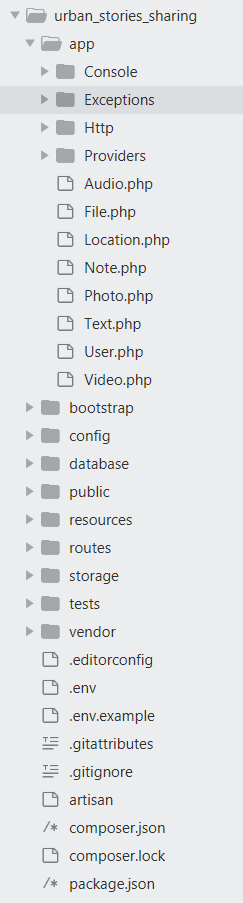
\includegraphics[width=0.2\linewidth, height=0.4\textheight]{Struttura_applicazione}
	\caption{Struttura dell'applicazione}
	\label{fig:AppStructure}
\end{figure}


La struttura dell'applicazione lato back-end, visibile in figura \ref{fig:AppStructure}, mantiene la struttura base di un'applicazione Laravel, strutturata in cartelle, ognuna delle quali contiene dei files con uno specifico compito.

\subsection{App directory}
\begin{figure}[H]
	\centering
	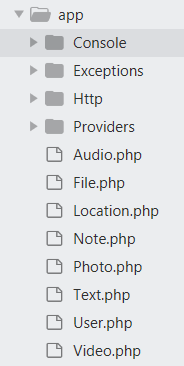
\includegraphics[width=0.15\linewidth, height=0.2\textheight]{AppDirectory}
	\caption{App directory}
	\label{fig:AppDirectory}
\end{figure}
La cartella \textit{\textbf{app}}, visibile in figura \ref{fig:AppDirectory}, contiene il codice principale dell'applicazione. Per impostazione predefinita del framework, questa directory è assegnata sotto il namespace di \textit{\textbf{App}} e viene caricata automaticamente da Composer.
Questa directory contiene tutti i modelli definiti per lo sviluppo del progetto oltre a varie sotto directory aggiuntive come Console e Http, che si possono considerare come un vero e proprio strato che fornisce un'API nel nucleo dell'applicazione.
La directory Console contiene tutti i comandi Artisan personalizzati, mentre la directory Http contiene controller e middleware, ovvero tutta logica per gestire le richieste.

\subsection{Database directory}
\begin{figure}[H]
	\centering
	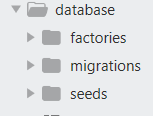
\includegraphics[width=0.2\linewidth, height=0.1\textheight]{DatabaseDirectory}
	\caption{Database directory}
	\label{fig:DBDirectory}
\end{figure}

La directory \textit{\textbf{Database}}, visibile in figura \ref{fig:DBDirectory}, contiene le migrazioni della base di dati e i file di \textit{\textbf{seeds}}, utili a popolare il modello.

\subsection{Storage directory}
La directory di archiviazione contiene l'archivio \textit{\textbf{/app/directory}} pubblico, il quale, viene utilizzato per archiviare file generati dall'utente, ovvero le note contenenti i file multimediali, che devono essere accessibili al pubblico. 
\vspace{-9px}
\section{Implementazione database}
Inizialmente, per quanto concerne la creazione del modello relazione, si era pensato di predisporre una entità autonoma per ogni tipo di file multimediale da caricare sul database, ma questo tipo di soluzione risultava ridondante poichè diverse entità presentavano gli stessi attributi, per questo motivo si è deciso di cambiare approccio e utilizzare un'entità genitore \textit{\textbf{files}}, si veda Listato \ref{lst:FilesSchema}, contenente le informazioni comuni, in relazione alle entità specializzanti per ogni tipo di file: \textit{\textbf{photos}}, \textit{\textbf{audios}} e \textit{\textbf{videos}}, visibili nel listato \ref{lst:VideosSchema}. 
\begin{lstlisting}[caption = Esempio schema tabella files, label={lst:FilesSchema}]
public function up()
{
	Schema::create('files', function (Blueprint $table) 
	{
		$table->increments('id');
		$table->float('size');
		$table->text('format');
		$table->mediumText('path')->nullable();
		$table->integer('note_id')->unsigned();
		$table->integer('photo_id')->unsigned()
			->unique()->nullable();
		$table->integer('audio_id')->unsigned()
			->unique()->nullable();
		$table->integer('video_id')->unsigned()
			->unique()->nullable();
		$table->foreign('note_id')->references('id')
			->on('notes');
		$table->foreign('photo_id')->references('id')
			->on('photos');
		$table->foreign('audio_id')->references('id')
			->on('audios');
		$table->foreign('video_id')->references('id')
			->on('videos');
		$table->timestamps();
	});
}
\end{lstlisting}
\pagebreak
\begin{lstlisting}[caption=Esempio schema tabella videos, label={lst:VideosSchema}]
public function up()
{
	Schema::create('videos', function (Blueprint $table) 
	{
		$table->increments('id');
		$table->integer('duration');
		$table->integer('width');
		$table->integer('height');
		$table->integer('bit_rate');
		$table->integer('frame_rate');
		$table->timestamps();
	});
}
\end{lstlisting}
Con lo sviluppo del progetto si è deciso di aggiungere, al modello, una nuova entità \textit{\textbf{notes}} messa in relazione con l'entità \textit{\textbf{files}}, \textit{\textbf{texts}} e \textit{\textbf{locations}}, rappresentante la geolocalizzazione delle note, che inizialmente era in relazione con l'entità \textit{\textbf{files}}.

\subsection{Codifica dei dati}
La codifica dei dati è un punto critico del progetto, poichè una scelta implementativa non ottimale potrebbe appensantire molto la base di dati.
Le due alternative possibili erano l'upload tramite \textit{\textbf{multipart form-data}} oppure tramite la \textit{\textbf{codifica in base64}}.

Dopo un'analisi delle ipotetiche dimensioni dei file salvate nel repository, si è scelto di riceve i dati codificati in \textit{\textbf{Base64}}, poiché si presuppone che le note testuali, le immagini, i file audio e i file video caricati sul server siano di piccole dimensioni.
Inoltre è stato scelto di non salvare la codifica dei dati nel database, per evitare, una volta raggiunti volumi importanti di dati, di appesantire la base di dati.
Per permettere, nonostante ciò, al client, di ricevere il file richiesto con \textit{\textbf{richieste HTTP}} di tipo \textit{\textbf{GET}}, il server si preoccupa di codificare i dati prima di essere inviati al client.

\pagebreak
\section{Implementazione web service}

Questa sezione tratta dell'implementazione del web service sviluppato per lo scambio di informazioni con la parte client, in particolare si mostrerà come vengono salvati e recuperati i file.

\subsection{Routes}

\begin{lstlisting}[caption={Definizione routes}, label={lst:RoutesDef}]
	Route::middleware('api');
	Route::get('/notes', 'NoteController@index');
	Route::get('/notes/{id}', 'NoteController@show');
	Route::get('/texts/{id}', 'TextController@show');
	Route::post('/texts', 'TextController@store');
	Route::get('/photos/{id}', 'PhotoController@show');
	Route::post('/photos', 'PhotoController@store');
	Route::get('/audios/{id}', 'AudioController@show');
	Route::post('/audios', 'AudioController@store');
	Route::get('/files/{id}', 'FileController@show');
	Route::get('/videos/{id}', 'VideoController@show');
	Route::post('/videos', 'VideoController@store');
\end{lstlisting}

Le routes, definite nel listato \ref{lst:RoutesDef}, vengono caricate dal \textit{\textbf{RouteServiceProvider}} a cui è assegnato il gruppo middleware 'api' e si occupano di instradare le richieste sui vari endpoint verso il controller dedicato.

\subsection{Controllers}

Definite le routes, sono stati realizzati i vari controller. Per ogni tipologia di file caricabile è stato definito un controller che gestisce le varie operazioni di richiesta e salvataggio dati.
Per ogni controller, quindi, sono stati definiti gli opportuni metodi che gestiscono le varie richieste HTTP;
i nomi dei metodi definiti all'interno dei controller sono stati standardizzati in modo da permettere una più semplice comprensione.

\pagebreak
\subsubsection{Metodo Index}
Il metodo \textit{\textbf{index}}, all'interno di un controller, risponde ad una richiesta di tipo \textit{\textbf{GET}} e si occupa di recuperare i file richiesti dal database. Il metodo può restituire una collezione di oggetti specifici, identificati dai parametri passati tramite query string oppure una collezione di tutte le note registrate nel database. Un esempio è riportato nel listato \ref{lst:NoteController@index}.

\begin{lstlisting}[caption={Funzione \textit{\textbf{index}} del controller NoteController},label={lst:NoteController@index}]
public function index(Request $request) {
	
	if($request->has('lat') &&
	$request->has('long')) {
	
		//Gestione dei parametri in query string
		
		return $notes;
	}
	if($request->has('type')) {

		//Gestione dei parametri in query string	
		
		return $notes;
	}
	return Note::All();
}
\end{lstlisting}

\subsubsection{Metodo Store}
Il metodo \textit{\textbf{store}} si occupa della gestione delle richieste HTTP di tipo \textit{\textbf{POST}}. 
Ovvero gestisce tutte le operazioni di salvataggio di ogni tipo di files \citep{rif2}\citep{rif4}.
Un esempio di \textit{\textbf{store}} è riportato nel listato \ref{lst:storeVideo}.

\pagebreak
\subsubsection{Metodo Show}
\begin{lstlisting}[caption={Funzione \textit{\textbf{show}} del controller NoteController}, label={lst:NoteController@show}]
public function show($id) 
{
	if(Note::find($id)){
		return Note::find($id);
	}else {
		return Response('Note not found', 404);
	}
}
\end{lstlisting}

Il un metodo \textit{\textbf{show}}, riportato nel listato \ref{lst:NoteController@show}, gestisce richieste HTTP di tipo \textit{\textbf{GET}} e ritorna un oggetto singolo che corrisponde ad un file, identificato dal parametro \textit{\textbf{id}} passato con la richiesta; il tipo dell'oggetto ritornato dipende dall'endpoint su cui si effettua la richiesta.

\subsubsection{Query string}
Quando viene effettuata una richiesta HTTP di tipo \textit{\textbf{GET}} può essere necessario passare dei parametri in \textit{\textbf{query string}} per specificare una certa tipologia di files da reperire.
Per permettere questo tipo di operazioni è stata implementata la gestione delle query string.
Sono stati previsti diversi tipi di parametri in input tramite query string. Il caso principale è quello di reperire delle note entro una certa distanza da una posizione data; per un esempio di chiamata con parametri in query string si può visionare il listato \ref{lst:QueryStringLocExample} presente in sezione \ref{sec:APIDocGetNotes}. 

La logica alla base di questa operazione, visibile nel listato \ref{lst:QueryStringLocation}, è quella di ottenere tutti i parametri passati in query string, ovvero le coordinate geografiche dell'utente e la distanza massima entro la quale si vogliono recuperare i dati; dopodichè, vengono ciclate tutte le note all'interno del repository e, sfruttando il teorema di Pitagora, vengono selezionate solo le note richieste.
\pagebreak
\begin{lstlisting}[caption={Recupero delle note entro una certa distanza da una posizione data}, label={lst:QueryStringLocation}]
foreach ($notes as $key => $value) {

	if($value->location != null) {
		$lat2 = $value->location->latitude;
		$long2 = $value->location->longitude;
		$distance = sqrt(
				pow($lat2-$lat1, 2) +
			 	pow($long2-$long1, 2)
			 	);

		if($distance > $max_distance) {
			$notes->forget($key);
		}    
	} else {
		$notes->forget($key);
	}
}
\end{lstlisting}
\pagebreak
Un altro esempio di richiesta \textit{\textbf{GET}} con parametri in query string è quello in cui si passa come parametro il tipo di file contenuto nelle note che si vuole reperire. Il codice che esegue questa operazione è riportato nel listato \ref{lst:QueryStringType}.

\begin{lstlisting}[caption={Recupero di un dato tipo di note},label={lst:QueryStringType}]
if($request->has('type')) {
	
	$request->validate([
	'type' => 'in:audio,photo,video,text'
	]);
	
	$queryStr = $request->query('type');
	$notes = collect();
	
	
	if($queryStr == 'text'){
		$texts = Text::All();
		foreach ($texts as $text) {
			$note = Note::find($text->note_id);
			$note->type = $queryStr;
			$note->content = $text->content;
			$notes->push($note);
		}
	return $notes;    
	}
	
	$files = File::whereNotNull($queryStr.'_id')->get();
	
	foreach ($files as $file) {
		$note = Note::find($file->id);
		$path = $file->path;
		$content = base64_encode(Storage::get($path));
		$note->type = $queryStr;
		$note->data = $content;
		$notes->push($note);
	}
	return $notes;
}
\end{lstlisting}

\pagebreak
\section{Archivio di salvataggio}
\begin{figure}[H]
	\centering
	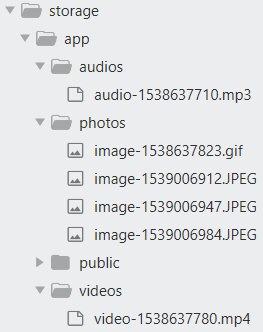
\includegraphics[width=0.3\linewidth, height=0.3\textheight]{StorageDirectory}
	\caption{Struttura directory storage}
	\label{fig:storageDirectory}
\end{figure}

L'ultima parte implementativa prevede la creazione dell'archivio in cui vengono salvati i files. Il salvataggio viene effettuato in locale e la collocazione è impostata nella directory \textit{\textbf{/storage/app/\begin{math}<\end{math}tipoFiles\begin{math}>\end{math}}} tramite i driver del disco locale.
Tutta la struttura della directory è riportata in figura \ref{fig:storageDirectory}. \\
In fase di salvataggio, dopo aver validato i parametri ricevuti in ingresso, viene generato il nome del file composto da \textit{\textbf{tipoFile-time.formatoFile}}.
Nel listato \ref{lst:storeVideo} è riportato un esempio di salvataggio di un file multimediale di tipo video.

\pagebreak
\begin{lstlisting}[caption={Esempio di salvataggio di un file video}, label={lst:storeVideo}]
public function store(Request $request)
	{
	
	//Validazione dell'input
	$validatedData = $request->validate([
		'size' => 'required|numeric',
		'format' => 'required|alpha_num',
		'duration' => 'required|numeric',
		'width' => 'required|numeric',
		'height' => 'required|numeric',
		'bit_rate' => 'required|numeric',
		'frame_rate' => 'required|numeric',
		'video_data' => 'required',
		'latitude' => 'required|numeric',
		'longitude' => 'required|numeric',
	]);
	
	//Preparazioni istanze per riempimento database record
	$video = new Video;
	$file = new File;
	$location = new Location;
	$note = new Note;
	
	//Preparazioni parametri di salvataggio
	$filename = 'video-'.time().'.'.$request['format'];
	$video_data = $request['video_data'];
	$fullPath = 'videos/'.$filename;
	
	Storage::disk('local')
		->put($fullPath, base64_decode($video_data));
	
	//Operazioni di riempimento database record
	
	return Response(['id' => $note->id], 201);
}
\end{lstlisting}



	\chapter{Risultati ottenuti e conclusioni}
In quest'ultimo capitolo vengono presentati i risultati ottenuti e i possibili miglioramenti per un possibile sviluppo futuro del progetto.



\section{Risultati ottenuti}
Il lavoro svolto durante questo progetto di stage ha permesso di ottenere un repository in grado di inviare e ricevere dati multimediali in formato JSON codificati in base64 da e verso un qualsiasi tipo di client, rispettando le direttive delle API sviluppate e descritte nel capitolo 3. 

\subsection{Ricezione dei dati}
Dal punto di vista della ricezione dei dati, il sistema, è in grado di ricevere qualsiasi file multimediale sottoforma di oggetti JSON e salvarli logicamente nel database creato e fisicamente sull'ipotetico server che ospiterà il web service.

\subsection{Invio dei dati}
Per quanto riguarda l'invio dei dati, invece, tramite le query descritte nel Capitolo 3, il sistema può recuperare tutti i dati salvati, genericamente oppure in base al tipo di file. Inoltre, si possono reperire note in base alla loro geolocalizzazione o richiedere files entro una certa distanza dalla posizione dell'utente.

\pagebreak
\section{Conclusioni}
Dall'analisi del risultato finale ottenuto viene compreso come il lavoro fin'ora prodotto sia funzionante ma migliorabile. 
Ad esempio, si potrebbe implementare la possibilità di gestire l'utenza, quindi aggiungere un servizio di autenticazione che permetta all'utente finale di avere uno storico dei file postati da esso o ancora di poter reperire informazioni riguardo le note postate dagli amici degli utenti. Questo prevede una riprogettazione del modello relazionale, poichè, allo stato attuale non è stato predisposto per questo tipo di funzioni.

Un altro aspetto migliorabile del web service è il lato della sicurezza dei dati, non gestito durante questo progetto.
Molti altri aspetti sono migliorabili o modificabili in base al tipo di client frontend, ancora in fase di progettazione, che verrà sviluppato in futuro.
	
	\backmatter
	% bibliography, glossary and index would go here.
	\renewcommand\bibname{Sitografia}
	\begin{thebibliography}{100}

		\bibitem{rif2} Bitfumes Webnologies, Youtube - Laravel 5.4 File upload - Save File to Database 7/9 \\
		\url{https://www.youtube.com/watch?v=7ZGFWvunoxw}	
		
		\bibitem{rif1} Dunebook - Inserting and updating related models in laravel \\
		\url{https://www.dunebook.com/inserting-and-updating-related-models-in-laravel-5-1/1/}
	
		\bibitem{rif7} Laracasts - Laracasts \\
		\url{https://laracasts.com/}	
		
		\bibitem{rif6} Laracast - Laravel from scratch \\
		\url{https://laracasts.com/series/laravel-from-scratch-2017}
		
		\bibitem{rif5} Laravel - Documentazione Laravel\\
		\url{https://laravel.com/docs/5.7}
	
		\bibitem{rif3} PHP - Documentazione PHP \\
		\url{http://it2.php.net/manual/en/}
	
		\bibitem{rif10} Stackoverflow - Custom created\_at and use only custom created\_at \\
		\url{https://stackoverflow.com/questions/47989148/custom-created-at-and-use-only-custom-created-at}
		
		\bibitem{rif4} Stackoverflow - Laravel 5.5 storing image from base64 string \\
		\url{https://stackoverflow.com/questions/49670746/laravel-5-5-storing-image-from-base64-string}
		
		\bibitem{rif9} Stackoverflow - Laravel eloquent nested query \\
		\url{https://stackoverflow.com/questions/29751104/laravel-eloquent-nested-query}
	
		\bibitem{rif11} Wikipedia - Application programming interface \\ \url{http://it.wikipedia.org/w/index.php?title=Application_programming_interface&oldid=99270655}
	
		\bibitem{rif8} Wikipedia - Modello entità-relazione \\
		\url{https://it.wikipedia.org/wiki/Modello_E-R#I_costrutti_principali_del_modello		}
	\end{thebibliography}
	
\end{document}